\subsection{Evolución Diferencia: Conceptos Básicos}

Esta sección esta dedicada para repasar la variante clásica de \DE{} y para introducir algunos de los mas importantes términos utilizados en el campo de \DE{}.
%This section is devoted to summarize the classic \DE{} variant and to introduce some of the most important terms used in the \DE{} field.
%
El clásico esquema \DE{} es identificado como \DE{}/rand/1/bin el cual ha sido extensamente utilizado para generar más variantes complejas~\cite{das2011differential}.
%The classic \DE{} scheme is called the \DE{}/rand/1/bin and it has been extensively used to generate more complex \DE{} variants~\cite{das2011differential}.
%
De hecho, nuestra propuesta también extiende a la clásica versión \DE{}.
%In fact, our proposal also extends the classic variant.
%
Originalmente \DE{} fue propuesta como un método de búsqueda directo para optimización contínua mono-objetivo.
%\DE{} was originally proposed as a direct search method for single-objective continuous optimization.
%
El conjunto de variables involucradas en el planteamiento de un problema son dados como un vector de la forma $\vec{X} = [x_1, x_2, ..., x_D]$, donde $D$ es la dimensión del problema.
%The variables governing a given problem performance are given as a vector like $\vec{X} = [x_1, x_2, ..., x_D]$, where $D$ is the
%dimension of the problem.
%
En optimización contínua, cada $x_i$ es un número real, además son proporcionadas restricciones de caja, es decir, existe un límite inferior ($a_{i}$) y un límite superior ($b_{i}$) para cada variable.
%In continuous optimization, each $x_i$ is a real number and usually box-constraints are given, i.e. there is a lower bound ($a_{i}$) and
%upper bound ($b_{i}$) for each variable.
%
El objetivo de un proceso de optimización es obtener un vector $\vec{X}^*$ el cual minimiza una función objetivo dada, esto matemáticamente es definido por $f : \Omega \subseteq \Re^D \rightarrow \Re$.
%The aim of the optimization process is to obtain the vector $\vec{X}^*$ which minimizes a given objective function, mathematically 
%denoted by $f : \Omega \subseteq \Re^D \rightarrow \Re$.
%
En el caso de la restricción de caja $\Omega = {\prod}_{j=1}^{D} [a_{j}, b_{j}]$.

%In the box-constrained case $\Omega = {\prod}_{j=1}^{D} [a_{j}, b_{j}]$.
\DE{} es un algoritmo estocástico basado en una población, por lo tanto éste involucra iterativamente a un conjunto de soluciones candidatas.
%\DE{} is a population-based stochastic algorithm, so it iteratively evolves a set of candidate solutions.
%
En \DE{} dichas soluciones candidatas son usualmente conocidas como vectores.
%In \DE{} such candidate solutions are usually called vectors.
%
En la variante básica de \DE{}, para cada miembro de la población conocidos como \textit{vectores objetivo} es generado un nuevo vector conocido como \textit{vector mutado}.
%In the basic \DE{} variant for each member of the population --- they are called \textit{target vectors} --- a new \textit{mutant vector}
%is created.
%
Entonces, el vector mutado es combinado con el vector objetivo para generar al \textit{vector de prueba}.
%Then, the mutant vector is combined with the target vector to generate a \textit{trial vector}.
%
Finalmente, una fase de selección es aplicada para seleccionar a los vectores sobrevivientes.
%Finally, a selection phase is applied to choose the survivors.
%
De esta forma, transcurren las generaciones hasta cumplir el criterio de paro.
%In this way, several generations are evolved until a stopping criterion is reached.
%
El $i$-ésimo vector de la población en la generación $G$ es definido como$\vec{X}_{i,G} = [x_{1,i,G}, x_{2,i,G},..., X_{D,i, G}]$.
%The $i$th vector of the population at the generation $G$ is denoted as $\vec{X}_{i,G} = [x_{1,i,G}, x_{2,i,G},..., X_{D,i, G}]$.
%
A continuación se explica en más detalle cada componente de \DE{}.
%In the following more details are given for each component of \DE{}.


\subsubsection{Inicialización}

\DE{} usually starts the optimization process with a randomly initiated population of $NP$ vectors.
%
Since there is commonly no information about the performance of different regions, uniform random generators are usually applied.
%
Hence, the $j$th component of the $i$th vector is initialized as $x_{j,i,0} = a_{j} + rand_{i,j}[0,1] (b_{j} - a_{j})$,
where $rand_{i,j}[0,1]$ is an uniformly distributed random number lying between $0$ and $1$.

\subsubsection{Mutación}

Para cada vector objetivo un vector mutado es creado, varias estratigias para realizar este procedimiento han sido propuestas.
%For each target vector a mutant vector is created and several ways of performing
%such a process have been proposed.
%
En la variante clásica de \DE{} se aplica la estrategia rand/1.
%In the classic \DE{} variant the rand/1 strategy is applied.
%
En este caso, es creado el vector mutado $V_{i,G}$ de la siguiente forma:
%In this case, the mutant vector $V_{i,G}$ is created as follows:

\begin{equation}\label{eqn:mutation}
\vec{V}_{i,G} = \vec{X}_{r1, G} + F \times (\vec{X}_{r2, G} - \vec{X}_{r3, G}) \quad r1 \neq r2 \neq r3
\end{equation}
%
Los índices $r1, r2, r3 \in [1,NP]$ distintos enteros seleccionados de forma aleatoria en el rango $[1, NP]$.
%The indices $r1, r2, r3 \in [1,NP]$ are different integers randomly chosen from the range $[1, NP]$.
%
Además, estos índices son distintos al índice $i$.
%In addition, they are all different from the index $i$.
%
Es imporante tomar en cuenta que la diferencia entre los vectores es escalada por medio del parámetro $F$, el cual se define usualmente en el intérvalo $[0.4, 1]$.
%It is important to take into account that the difference between vectors is scaled with the number F, which is usually defined in the interval $[0.4, 1]$.
%
La diferencia escalada es agregada al tercer vector, por lo tanto los vectores mutados son similares a los vectores objetivo cuando el grado de diversidad es poco y las diferencias son pequeñas.
%The scaled difference is added to a third vector, meaning that
%when diversity decreases and consequently differences are low, mutant vectors are similar to target vectors.
%
Como resultado, es importante mantener un grado de diversidad mínimo en \DE{}.
%As a result, maintaining some degree of diversity is specially important in \DE{}.

\subsubsection{Cruza}

En orden con el objetivo de combinar la información de distintas soluciones candiadtas y con el propósito de incrementar la diversidad es aplicado el operador de cruce.
%In order to combine information of different candidate solutions and with the aim of increasing diversity, the crossover
%operator is applied.
%
Específicamente, cada vector objetivo $\vec{X}_{i,G}$ es mezclado con su correspondiente vector mutado $V_{i,G}$ para general un vector de prueba $\vec{U_{i,G}} = [u_{1,i,G},u_{2,i,G}, ..., u_{D,i,G} ]$.
%Specifically, each target vector $\vec{X}_{i,G}$ is mixed with its corresponding mutant vector $V_{i,G}$ to 
%generate the trial vector $\vec{U_{i,G}} = [u_{1,i,G},u_{2,i,G}, ..., u_{D,i,G} ]$.
%
La estrategia de cruza mas típica es conocida como cruza \textit{binomial}, el cual funciona de la siguiente forma:
%The most typical crossover is the \textit{binomial} one, which operates as follows:
%
\begin{equation} \label{eqn:crossover}
\vec{U}_{j,i,G}= 
\begin{cases}
    \vec{V}_{j,i,G},& \text{si} (rand_{i,j}[0,1] \leq CR \quad or \quad j = j_{rand}  )\\
    \vec{X}_{j,i,G},              & \text{de otra forma}
\end{cases}
\end{equation}
donde $rand_{i,j}[0,1]$ es un número uniformemente distribuido, $j_{rand}$ es un índice aleatoriamente seleccionado el cual asegura que $\vec{U}_{i,G}$ genera al menos un componente de $\vec{V}_{i,G}$ y $CR \in [0,1]$ es la razón de cruce.
%where $rand_{i,j}[0,1]$ is a uniformly distributed random number,
%$j_{rand}$ is a randomly chosen index which ensures that $\vec{U}_{i,G}$ inherits at least one component from $\vec{V}_{i,G}$ and
%$CR \in [0,1]$ is the crossover rate.


\subsubsection{Selección}
Finalmente, se aplica una selección glotona para determinar a los sobreviviente de la siguiente generación.
%Finally, a greedy selection is performed to determine the survivors of the next generation.
%
Cada vector de prueba es comparado con su correspondiente vector objetivo y el mejor es el que sobrevive:
%Each trial vector is compared with its corresponding target vector and the best one survives:

\begin{equation} \label{eqn:selection}
\vec{X}_{j,i,G+1}= 
\begin{cases}
    \vec{U}_{i,G},& \text{si} \quad f(\vec{U}_{i,G}) \leq f(\vec{X}_{i,G})  \\
    \vec{X}_{i,G},              & \text{de otra forma}
\end{cases}
\end{equation}

Hence, each population member either gets better or remains with the same objective value in each generation.
%
Since members never deteriorate, it is considered to be a selection with high pressure.
%
Note that in case of a tie, the trial vector survives.

%
%The general convention is DE/\textit{x}/\textit{y}/\textit{x}, where DE indicates ``Differential Evolution'', \textit{x} denotes the base vector to be perturbed, \textit{y} is the number of difference vectors considered for perturbation and \textit{z} is the type of crossover to use.

\subsection{Diversidad en Evolución Diferencial}
%\subsection{Diversity in Differential Evolution}

Los algoritmos basados en \DE{} son altamente suceptibles a la pérdida de diversidad devido a la estrategia de selección agresiva.
%\DE{} is highly susceptible to the loss of diversity due to the greedy strategy applied in the selection phase.
%
Sin embargo, se han desarrollado varios análisis para lidiar con este problema.
%However, several analyses to better deal with this issue have been carried out.
%
Desde que se conocen las implicaciones de cada parámetro en la diversidad, una alternativa es la estimación teórica de los valores adecuados en \DE{}~\cite{zaharie2003control}.
%Since the general implications of each parameter on the diversity are known, one of
%the alternatives is to theoretically estimate proper values for the \DE{} parameters~\cite{zaharie2003control}.
%
Alternativamente, se han desarrollado algunos análisis donde es considerado el efecto de los vectores de diferencia en la mutación~\cite{montgomery2009differential}.
%Differently, some analyses regarding the effects of the norm of the difference vectors used in the mutation
%have also been performed~\cite{montgomery2009differential}.
%
Estos análisis y otros estudios empíricos basados en la cruza permitieron concluir que ciertos tipos de movimientos deberían ser deshabilidatos para retrasar la convergencia~\cite{montgomery2012simple}.
%Such analyses and additional empirical studies regarding the crossover allowed to conclude that some kind of movements 
%might be disallowed to delay the convergence~\cite{montgomery2012simple}.
%
En este último estudio varía el tipo de movimientos aceptados a lo largo de la ejecución.
%In this last study the kind of accepted movements varies along the run.
%
Específicamente, esto descarta movimientos menores a un umbral el cual es decrementado conforme transcurren las generaciones.
%Specifically, it discards movements with a size below a threshold and this threshold decreases taking into account the elapsed generations.
%
Se han propuesto otras formas de alterar el procedimiento en que se aceptan los movimientos~\cite{bolufe2013differential}.
%Other ways of altering the kind of accepted movements have been proposed~\cite{bolufe2013differential}.
%
Es importante notar que este tipo de métodos tienen similitudes con nuestra propuesta en el sentido de que las decisiones están basadas por el número de generaciones transcurridas.
%Note that these kinds of methods have similarities with our proposal in the sense that decisions are biased by the number of elapsed generations.
%
Sin embargo, nuestro método opera en la estrategia de reemplazo y no en la fase de mutación.
%However, our method operates on the replacement strategy and not on the mutation phase.
%
Mas aún, estos métodos no consideran de forma explícita las diferencias que aparecen en la población entera.
%Moreover, these methods do not consider explicitly the differences appearing on the whole population.
%
En su lugar, las restricciones son aplicadas a las diferencias que aparecen en la fase de reemplazo.
%Instead, the restrictions apply to the differences appearing in the reproduction phase.

Una alternativa distinta reside en alterar el operador de selección~\cite{sa2008exploration}.
%A different alternative operates by altering the selection operator~\cite{sa2008exploration}.
%
Particularmente, se relaja la presión de selección a través de una selección probabilística con el propósito de mantener la diversidad en la población y consecuentemente permitir escapar de la base de atracción de un óptimo local.
%Particularly, the selection pressure is relaxed through a probabilistic selection to maintain the population diversity and consequently 
%to allow escaping from basin of attraction of local optima.
%
Sin embargo este método es muy sensible a transformaciones desde que esta estrategia considera la aptitud para definir las probabilidades para aceptar un individuo mutado.
%Since it considers the fitness to establish the acceptance probabilities, it is very sensitive to scale transformations.
%
En este caso las decisiones no se basan en las generaciones transcurridas.
%In this case, decisions are not biased by the elapsed generations.

Finalmente, en el algoritmo \textit{Diversidad de la Población Auto-Mejorado} (\textit{Auto-Enhanced Population Diversity} - \textsc{aepd}), la diversidad es explícitamente medida y esto es un dispara un mecanismo para diversificar a la población cuando se detecta poca diversidad en la población~\cite{yang2015differential}.
%Finally, in the \textit{Auto-Enhanced Population Diversity} (\textsc{aepd}), the diversity is explicitly measured and it triggers a mechanism
%to diversify the population when a too low diversity is detected~\cite{yang2015differential}.
%
También ya se han propuesto estrategias con principios similares pero con esquemas de perturbación distintos.
%Strategies with similar principles but with different disturbance schemes have also been devised~\cite{zhao2016differential}.


Es importante notar que las mejores variantes-\DE{} de las competencias no utilizan estas modificaciones y que la mayoría de estas extensiones no han sido implementadas en los herramientas de optimización más utilizadas.
%Note that \DE{} variants with best performance in competitions do not apply these modifications
%and that most of these extensions have not been implemented in the most widely used frameworks.
%
Como resultado, estas extensiones no son ampliamente utilizadas por la comunidad a pesar de sus beneficios en ciertos casos.
%As a result, these extensions are not so widely used in the community in spite of their important benefits
%for some cases.


\subsection{Propuesta}

Nuestra propuesta está motivada por dos trabajos significativos de ésta área cuyo propósito es el control de la diversidad en los \EAS{}.
%Our proposal is motivated by two main works in the area of control of diversity in EAs.
%
Por su parte el primero es un estudio empírico desarrollado por Montgomery y otros~\cite{montgomery2012simple}, este trabajo presenta varios análisis empíricos los cuales confirman los problemas relacionados con la convergencia prematura.

%The first one is the empirical study developed by Montgomery et al~\cite{montgomery2012simple},
%which presents several empirical analyses that confirm issues related to premature convergence in \DE{}.
%
Por otro lado, el segundo trabajo propuesto por Segura~\cite{segura2016novel} y otros, proporciona mejoras significativas en el campo optimización combinatoria, en esta propuesta se desarrolla una novel estrategia de reemplazo nombrada \textit{Reemplazo con Control de Diversidad Dinámico Basado en Varios Objetivos} (Replacement with Multi-objective based Dynamic Diversity Control - \RMDDC{}) donde se controla el grado de diversidad con el criterio de paro y las generaciones transcurridas.
%The second work, by Segura et al.~\cite{segura2016novel}, provides significant improvements in the combinatorial optimization field
%by developing a novel replacement strategy called \textit{Replacement with Multi-objective based Dynamic Diversity Control} (\RMDDC{}) 
%that relates the control of diversity with the stopping criterion and elapsed generations.
%
Se obtuvieron beneficios por los métodos que incluyeron el \RMDDC{}, por lo tanto y basados en las conclusiones de los trabajos previos, la propuesta de esta sección es una novel variante de \DE{} que incluye un mecanismo explícito el cual sigue uno de los principios del \RMDDC{}.
%Important benefits were attained by methods including \RMDDC{}, so given the conclusions of these previous works, the proposal of this paper is a 
%novel \DE{} variant that includes an explicit mechanism that follows some of the principles of \RMDDC{}.
%
Este novel optimizador es nombrado \textit{Evolución Diferencial con Mantinimiento Mejorado de Diversidad} (Differential Evolution with Enhanced Diversity Maintenance - \DEEDM{}) y su código fuente está disponible de forma gratuita~\footnote{El código en C++ puede ser descargado en la siguiente dirección \url{https://github.com/joelchaconcastillo/Diversity\_DE\_Research.git} }
%This novel optimizer is called \textit{Differential Evolution with Enhanced Diversity Maintenance} (\DEEDM{}) and its source
%code is freely available~\footnote{The code in C++ can be downloaded in the next link \url{https://github.com/joelchaconcastillo/Diversity\_DE\_Research.git}}.


La escencia de \DEEDM{} (ver algoritmo~\ref{alg:DEEDM} ) es suficiente similar a la versión estándar de \DE{}.
%The core of \DEEDM{} (see Algorithm~\ref{alg:DEEDM}) is quite similar to the standard \DE{}.
%
De hecho la forma en que se crean los vectores de prueba no es modificado de forma significativa (líneas 5 y 6).
%In fact the way of creating new trial solutions is not modified at all (lines 5 and 6).
%
La novedad de la propuesta es que incorpora una población elite ($E$) y una novel estrategia de reemplazo basada en la diversidad.
%%The novelty is the incorporation of an elite population ($E$) and a novel diversity-based replacement strategy.
%
En orden, para seleccionar a los miembros de la población, se aplica el reemplazo agresivo (glotón) de la versión original de \DE (línea 7).
%In order to select the members of the elite population, the original greedy replacement of \DE{} is used (line 7).
%
Por otra parte, se considera otra estrategia de reemplazo (línea 8), la cual realiza la selección de los miembros que participarán en el siguiente procedimiento de selección, esto se realiza siguiendo el mismo principio que el \RMDDC{}, es decir los individuos que contribuyen muy poco a la diversidad no deberán ser aceptados como miembros en la siguiente generación.
%On the other way, the replacement strategy (line 8), which is in charge of selecting the next population members,
%follows the same principle that guided the 
%design of \RMDDC{}, i.e. individuals that contribute too little to diversity should not be accepted as members of the next generation.
%
En este sentido, no se utiliza la misma estrategia de selección agresiva que pertenece a \DE{} para mantener a la población padre ($X$).
%In this way, the greedy selection strategy of \DE{} is not used to maintain the parent population ($X$).
%
En este orden para establecer una contribución aceptable de diversidad mínima para realizar la selección, son tomados en cuenta el criterio de paro y las generaciones transcurridas.
%In order to establish the minimum acceptable diversity contribution to be selected, the stopping criterion and elapsed
%generations are taken into account.
%
Una de las principales debilidades del \RMDDC{} es que su convergencia se retrasa de forma significativa.
%One of the main weaknesses of \RMDDC{} is that its convergence is highly delayed.
%
Por lo tanto, se realizan dos modificaciones al \RMDDC{} para promover una convergencia acelerada.
%Thus, in order to promote a faster convergence than in \RMDDC{} two modifications are performed.
%
Primero, no son considerados los conceptos multi-objetivo, en su lugar se considera una selección mas agresiva.
%First, no concepts of the multi-objective field are applied, instead a more greedy selection is taken into account.
%
Segundo, también es considerada la población elite en  la estrategia de reemplazo.
%Second, the elite population is also considered as an input of the replacement strategy.

\begin{algorithm}[t]
\algsetup{linenosize=\tiny}
  \scriptsize
	\caption{Esquema general del DE-EDM} 
	%\caption{General scheme of DE-EDM} 
	\begin{algorithmic}[1]
	%\STATE Randomly initialize the population of $NP$ individuals, where each one is uniformly distributed.
	\STATE Inicializar de forma aleatoria a la población con $NP$ individuos, donde cada uno es distribuído de forma uniforme.
	\STATE $G=0$
	\WHILE{ El criterio de paro no sea alcanzado}
	%\WHILE{ stopping criterion is not satisfied}
	   \FOR{ $i=1$ to $NP$} 
		\STATE Mutación: Generar al vector mutado ($V_{i,G}$) de acuerdo a la ecuación (\ref{eqn:mutation}).
		%\STATE Mutation: Generate the mutant vector ($V_{i,G}$) according to Eq. (\ref{eqn:mutation}).
		\STATE Cruza: Utilizar la recombinación para general al vector de prueba ($U_{i,G}$) de acuerdo a la ecuación (\ref{eqn:crossover}).
		%\STATE Crossover: use recombination to generate the trial vector ($U_{i,G}$) according to Eq. (\ref{eqn:crossover}).
		\STATE Selección: Actualizar al vector elite ($E_{i,G}$ en lugar de $X_{i,G}$) de acuerdo a la ecuación (\ref{eqn:selection}).
		%\STATE Selection: Update the elite vector ($E_{i,G}$ instead of $X_{i,G}$) according to Eq. (\ref{eqn:selection}).
	   \ENDFOR
		\STATE Reemplazo: Seleccionar a los vectores objetivo ($X_{G+1}$) de acuerdo a la ecuación (\ref{alg:Replacement}).
		%\STATE Replacement: Select the target vectors ($X_{G+1}$) according to Algorithm \ref{alg:Replacement} .
	   \STATE $G=G+1$
	\ENDWHILE
\end{algorithmic}
    \label{alg:DEEDM}
\end{algorithm}


Nuestra estrategia de reemplazo (ver Algoritmo \ref{alg:Replacement}) funciona de la siguiente forma.
%Our replacement strategy (see Algorithm \ref{alg:Replacement}) operates as follows.
%
Éste recive a la población padre (vectores objetivo), la población de hijos (vectores de prueba) y a los vectores elite.
%It receives as input the parent population (target vectors), the offspring population (trial vectors), and the elite population.
%
En cada generación son seleccionados $NP$ vectores para la siguiente población de padres.
%In each generation it must select the $NP$ vectors of the next parent population.
%
Primero, en base al número de evaluaciones a funcion (línea 2) es calculada una distancia mínima $D_t$ deseada para mantener la diversidad.
%First, it calculates the desired minimum distance $D_t$ given the current number of elapsed function evaluations (line 2).
%
Entonces, son juntadas las tres poblaciones en un conjunto de miembros candidatos (línea 3).
%Then, it joins the three populations in a set of current members (line 3).
%
El conjunto de miembros candidatos continen vectores que podrían ser seleccionados para sobrevivir.
%The current members set contains vectors that might be selected to survive.
%
Entonces, el conjunto de individuos sobrevivientes y penalizados son inicializados por el conjunto vacío (línea 4).
%Then, the set of survivors and penalized individuals are initialized to the empty set (line 4).
%
En orden para seleccionar a los $NP$ sobreviviente (población padre de la siguiente generación) se repite un procedo iterativo (líneas 5 - 13).
%In order to select the $NP$ survivors (next parent population) an iterative process is repeated (lines 5 - 13).
%
En cada paso es seleccionado el mejor individuo para sobrevivir del \textit{Conjunto de Candidatos}, es decir al individuo que tiene la mejor aptitud, entonces es movido al \textit{Conjunto de Sobrevivientes}.
%In each step the best individual in the \textit{Current set}, i.e. the one with best objective function is selected
%to survive, i.e. it is moved to the \textit{Survivor set} (line 6 - 8).
%
Entonces, los individuos que pertenecen al \textit{Conjunto de Candidatos} cuya métrica de mínima distancia sea menor que $D_t$ son transferidos \textit{Conjunto de Penalizados} (línea 9).
%Then, individuals in the \textit{Current set} with a distance metric lower than $D_t$ are transferred to the \textit{Penalized set} (line 9).
%

La forma para calcular la distancia entre dos indivíduos es en base a la distancia Euclideana normalizada descrita en la ecuación~\ref{eqn:distance}, donde $D$ es la dimensión del problema, y $a_d, b_d$ son los límites menores y mayores de cada dimensión ($d$).
%The way to calculate the distance between two individuals is by using the normalized Euclidean distance described in Eq.~\ref{eqn:distance}, where $D$ is the dimension of the problem, and $a_d, b_d$ are the minimum and maximum bounds of each dimension ($d$).
%
%
En los casos donde \textit{El conjunto de Candidatos} está vacío previamente a la selcción de los $NP$ individuos, el \textit{Conjunto de Sobrevivientes} se llena seleccionando en cada iteración al individuo $Penalizado$ con la mayor distancia al individuo más cercano al \textit{Conjunto de Sobrevivientes} (líneas 10 - 13).
%%In cases where the \textit{Current set} is empty previous to the selection of $NP$ individuals, the \textit{Survivor set} is filled by selecting in each step 
%%the individual in $Penalized$ with the largest distance to the closest individual in the \textit{Survivor set} (lines 10 - 13).

\begin{equation}\label{eqn:distance}
distance ( x_{i}, x_j ) = \frac{\sqrt{ \sum_{d=1}^D \left ( \frac{x_{i}^d - x_j^d}{b_d - a_d} \right )^2  }} {\sqrt{D}}
\end{equation}


\begin{algorithm}[t]
\algsetup{linenosize=\tiny}
  \scriptsize
	\caption{Fase de Reemplazo} \label{alg:Replacement}
	%\caption{Replacement Phase} \label{alg:Replacement}
	\begin{algorithmic}[1]
	\STATE Entrada: \textit{Población} (\textit{Vectores Objetivo}), \textit{Hijos} (\textit{Vectores de prueba}), y \textit{Elite}
	%\STATE Input: $Population$ ($target$ $vectors$), $Offspring$ ($trial$ $vectors$), and $Elite$
	\STATE Actulizar $D_t = D_I - D_I *(nfes/(0.95*max\_nfes)) $ 
	%\STATE Update $D_t = D_I - D_I *(nfes/(0.95*max\_nfes)) $ 
	\STATE \textit{Candidatos = Población} $\cup$ \textit{Hijos} $\cup$ \textit{Elite}.
	%\STATE $Current = Population \cup Offspring \cup Elite$.
	\STATE \textit{Sobrevivientes} $=$ \textit{Penalizados} $\emptyset$.
	%\STATE $Survivors = Penalized = \emptyset$.
	\WHILE{ \textit{Sobrevivientes} $< NP$  y $|$\textit{Candidatos}$| > 0$ }
	%\WHILE{ $|Survivors| < NP$ And $|Current| > 0$ }
	   \STATE \textit{Seleccionados} = Seleccionar al mejor individuo de \textit{Candidatos}.
	   %\STATE $Selected$ = Select the best individual of $Current$.
		 \STATE Eliminar \textit{Seleccionado} de \textit{Candidatos}.
		 %\STATE Remove $Selected$ from $Current$.
	   \STATE Copias \textit{Seleccionado} a \textit{Sobrevivientes}.
	  % \STATE Copy $Selected$ to $Survivors$.
	   \STATE Encontrar los individuos de \textit{Candidatos} cuya distancia a \textit{Seleccionados} sea menor que $D_t$ y moverlos al \textit{Penalizados}. En esta parte se considera la distancia normalizada (Ecuación \ref{eqn:distance}).
	   %\STATE Find the individuals from $Current$ with a distance to $Selected$ lower than $D_t$ and move them to $Penalized$. Normalized distance is considered (Eq. \ref{eqn:distance}).
	\ENDWHILE
	\WHILE{ $|$\textit{Sobrevivientes}$| < NP$ }
	%\WHILE{ $|Survivors| < NP$ }
	   \STATE \textit{Seleccionado} = Seleccionar al individuo de \textit{Penalizados} con la mayor distancia al individuo mas cercano a \textit{Sobrevivientes}.
	   %\STATE $Selected$ = Select the individual from $Penalized$ with the largest distance to the closest individual in $Survivors$.
		 \STATE Eliminar \textit{Seleccionado} de \textit{Penalizados}.
		 %\STATE Remove $Selected$ from $Penalized$.
	   \STATE Copiar \textit{Seleccionado} a \textit{Sobrevivientes}
	   %\STATE Copy $Selected$ to $Survivors$.
	\ENDWHILE
  \RETURN $Survivors$
\end{algorithmic}
\end{algorithm}

En este orden con el propósito de completar la descripción es importante especificar la forma en que se calcula $D_t$ y el para actualizar a los individuos elite.
%In order to complete the description it is important to specify the way to calculate $D_t$ and the methodology to update the 
%elite individuals.
%
El resto del algortimo es mantenido de igual forma que la clásica variante de \DE{}.
%All the remaining steps are maintained as in the classic \DE{} variant.
%
El valor de $D_t$ es utilizado para alterar el grado entre exploración y explotación, por lo tanto éste parámetro debería depender en la etapa de optimización.
%The value of $D_t$ is used to alter the degree between exploration and explotation so it should depend on the optimization stage.
%
Específicamente, este valor debería se reducido conforme se alcanza el criterio de paro con el objetivo de promover un grado de intensificación.
%Specifically, this value should be reduced as the stopping criterion is reached with the aim of promoting explotation.
%
En nuestro esquema se requiere asignar un valor inicial para $D_t$ ($D_I$).
%In our scheme, an initial value for $D_t$ ($D_I$) must be set.
%
Así, similarmente que en~\cite{segura2016novel}, se calcula una reducción lineal de $D_t$ considerando las evoluciones a función y el criterio de paro, 
%Then, similarly than in~\cite{segura2016novel}, a linear reduction of $D_t$ is performed by taking into account the elapsed function evaluations and stopping criterion.
%
Particularmente, en este trabajo, el criterio de paro es asigna en base a las evaluaciones a función.
%Particularly, in this work, the stopping criterion is set by function evaluations.
%
La reducción es calculada de tal forma que en el $95\%$ del máximo número de evaluaciones a función el valor de $D_t$ es $0$.
%The reduction is calculated in such a way that by the $95\%$ of maximum number of evaluations the resulting $D_t$ value is $0$.
%
Por lo tanto, la diversidad no es considerada del todo en el restante $5\%$.
%Therefore, in the remaining $5\%$ diversity is not considered at all.
%
Entonces, si $max\_nfes$ es el máximo número de evaluaciones y $nfes$ es el número de evaluciones trascurridas $nfes$, entonces $D_t$ puede ser calculado de la siguiente forma $D_t=D_I - D_I *(nfes/(0.95*max\_nfes))$.
%Thus, if $max\_nfes$ is the maximum number of evaluations and $nfes$ is the elapsed number of evaluations, $D_t$ can be calculated as $D_t=D_I - D_I *(nfes/(0.95*max\_nfes))$.
%

La distancia inicial ($D_I$) afecta de forma considerable al rendimiento del \DEEDM{}.
%The initial distance ($D_I$) heavily affects the performance of \DEEDM{}.
%
Si este parámetro es elevado, entonces el algoritmo tiene como objetivo maximizar la diversidad de la población en las primeras etapas de optimización, por lo tanto se genera una exploración adecuada la cual es muy importante, particularmente en varios tipos de problemas tales como altamente multi-modales y deceptivos.
%If this parameter is fixed large enough, then at the first optimization stages the algorithm aims to maximize the diversity of the population, 
%so a proper exploration is performed which is very important in some kinds of problems such as highly multimodal and deceptive ones.
%
Entonces, se podría aliviar el efecto de la convergencia prematura.
%Thus, the effect of premature convergence might be alleviated.
%
Un valor muy elevado de $D_I$ podría inducir exploración excesivamente y por lo tanto una fase de intensificación podría no ser no es efectuada.
%A too large $D_I$ might induce too much exploration so a proper exploitation phase is not performed.
%
Por otra parte, un valor muy pequeño de $D_I$ podría evitar la fase de exploración, por lo tanto será más difícil evitar óptimos locales.
%In the opposite case, a too low $D_I$ might avoid the exploration phase, so avoiding local optima is more difficult.
%
El optimo $D_I$ podría variar dependiendo en el tipo problema y el criterio de paro.
%Depending on the kind of fitness landscape and stopping criterion, the optimal $D_I$ might vary.
%
En su lugar, los problemas deceptivos y altamente multi-modales usualmente requieren valores más elevados que en los problemas unimodales.
%For instance, deceptive and highly multi-modal problems usually require larger values than unimodal problems.
%
Sin embargo, en nuestra propuesta no se adapta un valor $D_I$ para cada problema, por lo tanto con el propósito de analizar la estabilidad de este parámetro se realiza un análisis con diferentes valores de $D_I$ en la sección de validación experimental.
%However, in our proposal, $D_I$ is not adapted to each problem, instead an experimental study to check the robustness
%of different $D_I$ value is attached in the experimental validation section. 
%

%
Al igual que a la versión estándar \DE{}, en nuestra propuesta \DEEDM{} se debe asignar una probabilidad de cruce ($CR$) y un factor de mutación ($F$).

%Similarly that the standard \DE{}, in \DEEDM{} the crossover probability ($CR$) and the mutation factor ($F$) must be set.
%
El primero es quizás es más importante de acuerdo a varios estudios desarrollados por Montgomery y otros \cite{montgomery2010analysis}.
%The first one is perhaps the most important for the performance according to several studies developed by Montgomery 
%et al. \cite{montgomery2010analysis}.
%
Estos autores probaron de forma empírica que valores extremos de $CR$ resultan en un comportamiento muy distinto.
%These authors empirically proved that extremes $CR$ values leads to vastly different search behaviors.
%
Ellos explicaron que bajos valores de $CR$ resultan en una búsqueda que es alineada con un pequeño número de ejes y además induce pequeños desplazamientos.
%They explained that low $CR$ values result in a search that is aligned with a small number of search space axes and
%induce small displacements.
%
Esto provoca una convergencia lenta y gradual que en algunos escenarios podría provocar un comportamiento robusto.
%This provokes a gradual and slow convergence that in some scenarios might result in a robust behavior.
%
Adicionalmente, valores elevados de $CR$ podrían generar soluciones de mayor calidad con una menor probabilidad.
%Additionally, high $CR$ values might generate higher quality solutions with a lower probability.
%
Sin embargo, estas transformaciones provocan largos desplazamientos que podrían mejorar de forma significativa.
%However, these transformations provoke large displacements that could improve significantly the solutions when successful.
%
De acuerdo a esto, en nuestra propuesta se emplean los dos principios, es decir, valores elevados y pequeños de $CR$ como es mostrado en la ecuación \ref{eqn:cr}.
%According to this, we employ both high and low $CR$ values as it is showed in Eq. \ref{eqn:cr}.

\begin{equation} \label{eqn:cr}
CR = 
\begin{cases}
     Normal(0.2, 0.1),& \text{si} \quad rand[0,1] \leq 0.5  \\
     Normal(0.9, 0.1),              & \text{de otra forma}
\end{cases}
\end{equation}

Siguiendo los principios de distintas variantes del SHADE~\cite{awad2016ensemble, brest2016shade}, se consideran las evaluaciones a función en el proceso de generación aleatorio del factor de mutación $F$.
%Following the principles of several SHADE variants~\cite{awad2016ensemble, brest2016shade}, the function evaluations are considered in the random generation of the mutation factor $F$.
%
Particularmente, cada valor $F$ es una muestra de una distribución Cauchy (Ecuación\ref{eqn:cauchy} ).
%Particularly, each $F$ is sampled through a Cauchy distribution (Eq. \ref{eqn:cauchy}).
\begin{equation}\label{eqn:cauchy}
 Cauchy(0.5, 0.5*nfes/max\_nfes)
\end{equation}
%
Por lo tanto, en las primeras etapas de optimización los valores de $F$ son generados de forma cercana a $0.5$.
%Therefore, at the first optimization stages, F values near to $0.5$ are generated.
%
Conforme la execución transcurre, la función de densidad sufre una transformación gradual donde la varianza se incremente, esto implica que son generados valores fuera del intérvalo $[0.0, 1.0]$ con una probabilidad alta.
%Then, as the execution advances, the density function suffers a gradual transformation and the variance is increased, meaning
%that values outside the interval $[0.0, 1.0]$ are generated with a higher probability.
%
En los casos cuando los valores son mayores a $1.0$, es utilizado un valor de $1.0$.
%In the cases when values larger than $1.0$ are generated, the value $1.0$ is used.
%
Si se genera un valor negativo, entonces este valor se vuelve a generar.
%In the case of generating a negative value, the $F$ is resampled.
%
Uno de los efectos de este enfoque es incrementar la probabilidad de generar valores elevados de $F$ conforme transcurren las generaciones con el objetivo de evitar una convergencia en las últimas etapas de optimización.
%One of the effects of this approach is to increase the probability of generating large $F$-values as the execution progresses
%with the aim of avoiding a fast convergence.



\subsection{Resultados}
En esta sección se presenta la validación experimental.
%In this section the experimental validation is presented.
%
Especialmente, demostramos que los resultados de los algoritmos que pertenecen al estado-del-arte pueden ser mejorados controlando explícitamente la diversidad en el clásico \DE{}.
%Specifically, we show that by explicitly controlling the diversity in DE, results of state-of-the-art algorithms
%are improved further.
%
Particularmente, se consideradon los conjuntos de prueba del \CEC{} 2016 y \CEC{} 2017.
%Particularly, the benchmarks of \CEC{} 2016 and \CEC{} 2017 are considered.
%
Cada uno está compuesto de treinta distintos problemas.
%Each one of them is composed of thirty different problems.
%
El estado-del-arte está compuesto por los algoritmos que alcanzaros los primeros lugares en cada año.
%The state-of-the-art is composed by the algorithms that attained the first places of each year competition.
%
Adicionalmente, se incluyó la versión estándar \DE{}.
%Additionally, the standard \DE{} was included.
%
Por lo tanto, los algoritmos considerados del \CEC{} 2016 son el UMOEAs-II~\cite{elsayed2016testing} y L-SHADE-EpSin \cite{awad2016ensemble}, los cuales alcanzaron el primero y el segundo lugar respectivamente.
%Thus, the algorithms considered from the \CEC{} 2016 are UMOEAs-II \cite{elsayed2016testing} and L-SHADE-EpSin \cite{awad2016ensemble} that achieved 
%the first and second place respectively.
%
Similarmente, los mejores algoritmos del \CEC{} 2017 son el EBOwithCMAR~\cite{kumar2017improving} y el jSO~\cite{brest2017single}.

%Similarly, the top algorithms from \CEC{} 2017 are EBOwithCMAR \cite{kumar2017improving} and jSO \cite{brest2017single}.
%
Es imporante destacar que el EBOwithCMAR es considerado como una mejora del UMOEAs-II.
%It is interesting to remark that EBOwithCMAR is considered as an improvement of the UMOEAs-II.
%
Adicionalmente, el jSO y el L-SHADE-EpSin pertenecen al a la familia de SHADE.
%Additionally, jSO and L-SHADE-EpSin belong to the SHADE's family.
%
Todos estos algoritmos fueron probados con los dos conjuntos de prueba como es sugeriodo en \cite{molina2017analysis}.
%All these algorithms are tested with both benchmarks as it is suggested by \cite{molina2017analysis}.
Debido a que todos los algoritmos son estocásticos se realizaron 51 ejecuciones con distintas semillas.
%Given that all of them are stochastic algorithms, each execution was repeated 51 times with different seeds.
%

En cada caso, el criterio de paso fue asignado a $25,000,000$ evaluaciones a función.
%In every case, the stopping criterion was set to $25,000,000$ functions evaluations.
%
La evaluación de los algoritmos se realizó siguiendo los lineamientos de las competencias del \CEC{}.
%We performed our evaluation following the guidelines of \CEC{} benchmark competitions.
%
Entonces, se asignó un error de $0$ si la diferencia entre la mejor solución encontrada y la solución óptima era menor que $10^{-8}$.
%Thus, if the gap between the values of the best solution found and the optimal solution was $10^{-8}$ or smaller, the error is treated as $0$.
%
%
Para cada algoritmo Se utilizó la parametrización indicada por los respectivos autores, que son definidos a continuación:
%The parameterization indicated by the authors was used in every algorithm and it is as follows:
\begin{itemize}
%\item \textbf{EBOwithCMAR}: For EBO, the maximum population size of $S_1 = 18D$, minimum population size of $S_1 = 4$, maximum population size of $S_2 = 146.8D$, minimum population size of $S_2 = 10$, historical memory size H=$6$. For CMAR Population size $S_3 = 4 + 3log(D)$, $\sigma=0.3$, CS = $50$, probability of local search $pl = 0.1$ and $cfe_{ls} = 0.4* FE_{max}$.
\item \textbf{EBOwithCMAR}: Para la parte EBO, el tamaño máximo de la población de $S_1 = 18D$, el tamaño mínimo de la población de $S_1 = 4$, el tamaño máximo de la población de $S_2 = 146.8D$, el tamaño mínimo de la población de $S_2 = 10$, el tamaño de la memoria histórica H=$6$. Para la parte de CMAR el tamaño de la población $S_3 = 4 + 3log(D)$, $\sigma=0.3$, CS = $50$, la probabilidad de búsqueda local $pl = 0.1$ y $cfe_{ls} = 0.4* FE_{max}$.
\item \textbf{UMOEAs-II}: Para la parte de MODE, el tamaño máxio de la población de $S_1 = 18D$, el tamaño mínimo de la població de $S_1 = 4$, el tamaño de la memoria histórica H=$6$. Para la parte del CMA-ES el tamaño de la población $S_2 = 4 + \lfloor 3log(D) \rfloor$, $\mu=\frac{PS}{2}$, $\sigma=0.3$, CS = $50$. Para la búsqueda local, $cfe_{ls} = 0.2 * FE_{max}$.
%\item \textbf{UMOEAs-II}: For MODE, maximum population size of $S_1 = 18D$, minimum population size of $S_1 = 4$, size memory H=$6$. For CMA-ES Population size $S_2 = 4 + \lfloor 3log(D) \rfloor$, $\mu=\frac{PS}{2}$, $\sigma=0.3$, CS = $50$. For local search, $cfe_{ls} = 0.2 * FE_{max}$.
\item \textbf{jSO}: El tamaño máximo de la población = $25log(D)\sqrt{D}$, el tamaño de la memoria histórica H= $5$, valor de mutación inicial de la memoria $M_F = 0.5$, probabilidad inicial de la memoria $M_{CR} = 0.8$, tamaño mínimo de la población = $4$, valor inicial p-best = $0.25*N$, valor final p-best = $2$.
%\item \textbf{jSO}: Maximum population size = $25log(D)\sqrt{D}$, historical memory size H= $5$, initial mutation memory $M_F = 0.5$, initial probability memory $M_{CR} = 0.8$, minimum population size = $4$, initial p-best = $0.25*N$, final p-best = $2$.
\item \textbf{L-SHADE-EpSin}: Tamaño máximo de la población = $25log(D)\sqrt{D}$, tamaño de la memoria histórica H= $5$, valor de la mutación inicial de la memoria $M_F = 0.5$, probabilidad inicial de la memoria $M_{CR} = 0.5$, frecuencia inicial de la memoria $\mu_F = 0.5$, tamaño mínimo de la población = $4$, valor inicial p-best = $0.25*N$, valor final p-best = $2$, generaciones de la búsqueda local $G_{LS}=250$.
%\item \textbf{L-SHADE-EpSin}: Maximum population size = $25log(D)\sqrt{D}$, historical memory size H= $5$, initial mutation memory $M_F = 0.5$, initial probability memory $M_{CR} = 0.5$, initial memory frequency $\mu_F = 0.5$, minimum population size = $4$, initial p-best = $0.25*N$, final p-best = $2$, generations of local search $G_{LS}=250$.
\item \textbf{ DE-EDM}: $D_I = 0.3$, tamaño de la población = $250$.
%\item \textbf{ DE-EDM}: $D_I = 0.3$, population size = $250$.
\item \textbf{ Standard-DE}: tamaño de la población = $250$ (mismos operadores que en \DEEDM{}).
\end{itemize}
%

Nuestro análisis experimental se desarrolló en base a la diferencia entre la solución óptima y la mejor solución obtenida.
%Our experimental analyses have been performed in base of the difference between the optimal solution and the best obtained solution.
%
En orden para comparar los resultados estadísticamente, se siguió un procedimiento similar que el propuesto en~\cite{Joel:StatisticalTest}.

%In order to statistically compare the results, a similar guideline than the one proposed in~\cite{Joel:StatisticalTest} was used. 
%
Concretamente, en primer lugar se utilizó el test Shapiro-Wilk para comprobar si los resultados se ajustaban a una distribución Gaussiana. 
%
En los casos en que sí se ajustaban, se utilizó el test de Levene para comprobar la homogeneidad de las varianzas, procediendo con el test de ANOVA en caso positivo o con el de Welch en caso negativo.
%
Por otro lado, para los casos que no se ajustaban a distribuciones Guassianas, se utilizó el test de Kruskal-Wallis.
%
En todos los casos se fijó el nivel de confianza al 95\%.
%
Se considera que un algoritmo $X$ es superior a un algoritmo $Y$, si el procedimiento anterior reporta diferencias significativas y si la media y mediana del hipervolumen obtenido por el método $X$ son superiores a las obtenidas por el método $Y$.
%
%First a Shapiro-Wilk test was performed to check whatever or not the values of the results followed a Gaussian distribution. 
%%
%If, so, the Levene test was used to check for the homogeneity of the variances. 
%%
%If samples had equal variance, an ANOVA test was done; if not, a Welch test was performed. 
%%
%For non-Gaussian distributions, the non parametric Kruskal-Wallis test was used to test whether samples are drawn from the same distribution. 
%%
%An algorithm $X$ is said to win algorithm $Y$ when the differences between them are statistically significant, and the mean and median obtained by $X$ are higher 
%than the mean and median achieved by $Y$.
En las tablas \ref{tab:Summary_CEC2016} y \ref{tab:Summary_CEC2017} se presenta un resúmen de los resultados obtenidos para el \CEC{} 2016 y el \CEC{} 2017 respectivamente.
%In tables \ref{tab:Summary_CEC2016} and \ref{tab:Summary_CEC2017} a summary of the results obtained for \CEC{} 2016 and \CEC{} 2017 are shown, respectively.
%
La columna etiquetada con ``Simpre Resuelto'' muestra el número de funciones en que se obtuvo un error de cero en las 51 ejecuciones.
%The column tagged with ``Always Solved'' shows the number of functions where a zero error was obtained in the 51 runs.
%
Adicionalmente, la columna etiquetada con ``Al menos una vez resuelto'' muestra el número de soluciones que se resolvieron en al menos una ejecución.
%Additionally, column tagged with ``At least one time solved'' shows the number of functions that were solved to optimality at least in one run.
%
Practicamente nuestra propuesta resolvió al menos una vez todas las funciones (28 funciones) que pertenecen al conjunto de problemas del \CEC{} 2017.
%Practically all functions (28 of them) of the \CEC{} 2017 benchmark were solved with our proposal at least one time.
%
Adicionalmente, fueron resueltas al menos una vez 21 funciones que pertenecen al \CEC{} 2016.
%Additionally, 21 functions of the \CEC{} 2016 were also solved.
%
Esta es una diferencia sustancial con los resultados obtenidos por los algoritmos que pertenecen al el estado-del-arte.
%This constrast with the results obtained by state-of-the-art algorithms.
%
Estos algoritmos obtuvieron los valores óptimos significativamente en menos funciones.
%They were able to reach optimal values in significantly less functions.
%
En orden para confirmar la superioridad del \DEEDM{}, se implementaron las pruebas estadísticas por pares.
%In order to confirm the superioriy of \DEEDM{}, pair-wise statisticall test were used.
%
La columna etiquetada con el símbolo $\uparrow$ muestra que el número de veces en que cada método fue superiror, mientras que la columna etiquetada con $\downarrow$ cuenta el número de casos donde el método fue inferior.
%The column tagged with the symbol $\uparrow$ shows the number of times that the superiority of each method could be confirmed, whereas
%the column tagged with the symbol $\downarrow$ count the number of cases where the method was inferior.
%
Finalmente, la columna etiquetada con $\longleftrightarrow$ muestra el número de comparaciones cuyas diferencias no fueron significativas.
%Finally, the number comparisons whose differences were not significant are shown in the column tagged with the symbol $\longleftrightarrow$.
%
%TODO: Poner frases del tipo que fue el que mas veces ganó y el que menos veces perdió
Las pruebas estadísticas indican que el \DEEDM{} alcanzó los mejores resultados en los dos años.
%The statistical tests indicate that the \DEEDM{} attained the best results in both years.
%
De hecho el número de veces en que nuestra propuesta ganó en el \CEC{} 2016 y el \CEC{} 2017 fue de $77$ y $88$ respectivemente.
%The number of wins in \CEC{} 2016 and \CEC{} 2017 were $77$ and $88$ respectively.
%
Además el número de veces en que perdió fueron de $25$ y $6$ respectivamente.
%Also the number of losts were of $25$ and $6$ respectively.
%
Adicionalmente, el último lugar alcanzado en los dos años  fue por el algoritmo L-SHADE-Epsilon con $20$ comparaciones positivas en el 2016 y $7$ comparaciones positivas en el 2017.
%Additionally, the last place attained in both years was by the L-SHADE-Epsilon with $20$ wins in 2016 and $7$ wins in 2017.
%
%
La última columna etiquetada con ``Puntaje'' muestra un análisis que fue propuesto en las competencias del \CEC{}.
%The last column tagget with ``Score'' shows the analyses proposed in the \CEC{}'s competitions.
%
Particularmente, este método de evaluación combina dos puntajes como se indica en la ecuación (\ref{eqn:total_scores}).
%Particularly, the evaluation method combines two scores defined in the equation (\ref{eqn:total_scores}).
%
%TODO: pasar el score a la última columna y decir que además del análisis se realizó el análisis propuesto en la competición, que se base
%en calcular un score...
%
Por lo tanto el puntaje final está compuesto por la suma $Score = Score_1 + Score_2$.

%Thus the final score is composed by the sum $Score = Score_1 + Score_2$.
%
\begin{equation}\label{eqn:total_scores}
\begin{split}
Score_1 &= \left (1 - \frac{SE - SE_{min}}{SE} \right) \times 50, \\
Score_2 &= \left  (1 - \frac{SR - SR_{min}}{SR} \right ) \times 50, \\
\end{split}
\end{equation}
donde, $SE_{min}$ es la suma mínima de errres entre todos los algoritmos, y $SE$ es la suma de errores dado un algoritmo $SE = \sum_{i=1}^{30} error\_f_i$.
%Here, $SE_{min}$ is the minimal sum of errors from all the algorithms, and $SE$ is the sum of error values $SE = \sum_{i=1}^{30} error\_f_i$.
%
Similarmente, $SR_{min}$ es la suma mínima de los rangos entre todos los algoritmos, especificamente es la suma de cada rango en cada función para los algoritmos considerados $SE = \sum_{i=1}^{30} error\_f_i$.
%Also, $SR_{min}$ is the minimal sum of ranks from all the algorithms, namely the sum of each rank in each function for the considered algorithms $SE = \sum_{i=1}^{30} error\_f_i$.
%
%TODO: remarcar que la nueva propuesta consigue score 100 en ambos casos, confirmando la superioridad que se vio con el resto de análisis realizados, decir
%que significa tener score 100
%
Principalmente, nuestra propuesta alcanzó los mejores puntajes ($100.00$) en los dos años, demostrando su superioridad. 
%Principally, our proposal attained the best scores ($100.00$) in both years, showing its superiority.
%
Adicionalmente, la versión estándar de \DE{} alcanzó resultados suficientemente buenos, de hecho obtuvo el tercer y el segundo lugar en los años 2016 y 2017 respectivamente.
%Additionally, the Standard-DE attained good enough results, in fact it got the third and second places in \CEC{} 2016 and \CEC{} 2017 respectively.
%
Esto muestra que el rendimiento de los algortimos en el-estado-del-arte es distinto al considerar ejecuciones a largo plazo.
%This shows that the performance of the state-of-the-art algorithms is different considering long-term executions.
%
El algoritmo L-SHADE-Epsilon obtuvo un puntaje competitivo a pesar de que en el \CEC{} del 2017  alcanzó el menor número de comparaciones positivas dentro de las pruebas estadísticas.
%Specifically, although that in \CEC{} 2017 the L-SHADE-Epsilon algorithm got the lowest number of wins in the statistical test it showed a competitive score.
%
Esto podría ocurrir desde que los puntajes estadísticos consideran la media y mediana de los errores.
%This might occurs since that the statistical scores considers both mean and median errors.
%
Es más el puntaje considera el rango y la media basado en el error.
%Morever, the score considers a rank and mean based in the error.
%

%TODO: Poner Dado que nuestra novedad está en el control de la diversidad, para comprender mejor el comportamiento de la propuesta...
Dado que nuestra propuesta está basada en el control explícito de la diversidad y con el objetivo de entender mejor su comportamiento, en la figura \ref{fig:diversity} se muestra la evolución de la diversidad a través de las evaluaciones a función.
%Giving that our proposal is based in the explicitly control of the diversity and with the aim of a better understanding of its behavior in the figure \ref{fig:diversity} is showed the diversity through the elapsed function evaluatons.
%
Particularmente, se ejecutó el \DEEDM{} con las funciones $F_1$ y $f_{30}$.
%Particularly, the \DEEDM{} was executed with the functions $f_1$ and $f_{30}$.
%
Basado en sus propiedades la primer función se resuelve de forma sencilla (unimodal) y la segunda función es considerada como una de las más difíciles (híbrida).
%Specifically, based in their properties the first function is easily solved (unimodal) and the second is one of the most difficult (hybrid).
%
En la parte izquierda se muestra la diversidad que se mantienen en la población Elite.
%In the left side is showed the diversity of the Elite population.
%
A pesar de que existen mecanismos para evitar la pérdida de diversidad en la población Elite, se puede observar que se mantiene un grado de diversidad de forma implícito en las dos funciones.
%Although there are not constraints in the Elite population to lost the diversity, it seems that in both functions $f_1$ and $f_{30}$ the diversity is implicitly maintained.
%
Similarmente, la parte derecha corresponde a la diversidad de los vectores de prueba.
%Similarly, in the right side is showed the diversity of the trial vectors.
%
Esto demuestra que se demuestra un grado de diversidad de forma explícito, es decir hasta el $95\%$ del total de evaluaciones a función.
%It shows that the diversity is explicitly maintained as is desired ( i.e. until the $95\%$ of the total function evaluations).

\begin{figure}[t]
\centering
\begin{tabular}{cc}
   \includegraphics[scale=0.23, angle=-90]{img/ED/Diversity_Elite.eps} 
   \includegraphics[scale=0.23, angle=-90]{img/ED/Diversity_Trial.eps} 
\end{tabular}
\caption{ Promedio del \DCN{} de las 51 ejecuciones con los problemas $f_1$ y $f_{30}$ (\CEC{} 2016 y \CEC{} 2017). El factor de distancia inicial corresponde a $D_I=0.3$.}
%\caption{ Average \DCN{} of the 51 executions with the problems $f_1$ and $f_{30}$ (\CEC{} 2016 and \CEC{} 2017). The initial distance factor considered corresponds to $D_I=0.3$.}
\label{fig:diversity}
\end{figure}


% Please add the following required packages to your document preamble:
% \usepackage{multirow}
\begin{table}[t]
\centering
\caption{Resúmen de los resultados - \CEC{} 2016}
\label{tab:Summary_CEC2016}
\begin{tabular}{|c|c|c|c|c|c|c|}
\hline
\multirow{2}{*}{\textbf{Algorithm}} & \multirow{2}{*}{\textbf{\begin{tabular}[c]{@{}c@{}}Siempre \\ Resuelto\end{tabular}}} & \multirow{2}{*}{\textbf{\begin{tabular}[c]{@{}c@{}}Resuelto al menos\\ una vez\end{tabular}}} & \multicolumn{3}{c|}{\textbf{Pruebas Estadísticas}} & \multirow{2}{*}{\textbf{Puntaje}} \\ \cline{4-6}
 &  &  & $\uparrow$ & $\downarrow$ & $\longleftrightarrow $ &  \\ \hline
\textbf{EBOwithCMAR} & 8 & 14 & 35 & 56 & 59 & 50.28 \\ \hline
\textbf{jSO} & 9 & 17 & 47 & 51 & 52 & 55.43 \\ \hline
\textbf{UMOEAs-II} & 9 & 14 & 51 & 31 & 68 & 62.45 \\ \hline
\textbf{L-SHADE-Epsilon} & 7 & 13 & 20 & 71 & 59 & 50.12 \\ \hline
\textbf{DE-EDM} & 13 & 21 & 77 & 25 & 48 & 100.00 \\ \hline
\textbf{Standard-DE} & 11 & 19 & 50 & 46 & 54 & 56.29 \\ \hline
\end{tabular}
\end{table}


% Please add the following required packages to your document preamble:
% \usepackage{multirow}
\begin{table}[t]
\centering
%\caption{Summary results - \CEC{} 2017}
\caption{Resúmen de los resultados - \CEC{} 2017}
\label{tab:Summary_CEC2017}
\begin{tabular}{|c|c|c|c|c|c|c|}
\hline
\multirow{2}{*}{\textbf{Algorithm}} & \multirow{2}{*}{\textbf{\begin{tabular}[c]{@{}c@{}}Siempre \\ Resuelto\end{tabular}}} & \multirow{2}{*}{\textbf{\begin{tabular}[c]{@{}c@{}}Resuelto al menos\\ una vez\end{tabular}}} & \multicolumn{3}{c|}{\textbf{Pruebas Estadísticas}} & \multirow{2}{*}{\textbf{Puntaje}} \\ \cline{4-6}
%\multirow{2}{*}{\textbf{Algorithm}} & \multirow{2}{*}{\textbf{\begin{tabular}[c]{@{}c@{}}Always \\ solved\end{tabular}}} & \multirow{2}{*}{\textbf{\begin{tabular}[c]{@{}c@{}}At least one\\ time solved\end{tabular}}} & \multicolumn{3}{c|}{\textbf{Statistical Tests}} & \multirow{2}{*}{\textbf{Score}} \\ \cline{4-6}
 &  &  & $\uparrow$ & $\downarrow$ & $\longleftrightarrow $ &  \\ \hline
\textbf{EBOwithCMAR} & 9 & 18 & 34 & 46 & 70 & 37.14 \\ \hline
\textbf{jSO} & 8 & 15 & 29 & 55 & 66 & 29.30 \\ \hline
\textbf{UMOEAs-II} & 11 & 15 & 43 & 40 & 67 & 26.89 \\ \hline
\textbf{L-SHADE-Epsilon} & 8 & 19 & 7 & 81 & 62 & 32.78 \\ \hline
\textbf{DE-EDM} & 21 & 28 & 88 & 6 & 56 & 100.00 \\ \hline
\textbf{Standard-DE} & 12 & 21 & 56 & 29 & 65 & 42.91 \\ \hline
\end{tabular}
\end{table}



%TODO: Con el fin de que otros autores se puedan comparar con los resultados, reportamos el error alcanzado
En orden, con el fin de proporcionar resultados comparables, en las tablas \ref{tab:Results_CEC2016} y \ref{tab:Results_CEC2017} se reporta el mejor, peor, mediana, media, desviación estándar y razón de éxito.
%In order, to provide comparable results of our proposal, in the tables \ref{tab:Results_CEC2016} and \ref{tab:Results_CEC2017} are reported the best, worst, median, mean, standard deviation and success ratio.
%
Particularmente, en estas tablas se observa que nuestra propuesta resuelve a todos los problemas unimodales.
%Particularly, these tables show that the uni-modal were solved by our proposal.
%
Además, varias funciones multimodales son aproximadas de forma aceptable.
%Also, several simple multi-modal functions were adequatelly approximated.
%
Principalmente, nuestra propuesta resolvió y mejoro significativamente varias funciones complejas (por ejemplo funciones computestas), que por otra parte no fueron resueltas por los algoritmos del estado-del-arte.
%Principally, our proposal solved several complex functions (e.g. Composition Functions) that were not solved by the state-of-the-art.
%
\begin{table}[t]
\begin{scriptsize}
\centering
\caption{Resultados del \DEEDM{} con los problemas del \CEC{} 2016}
%\caption{Results for DE based diversity \CEC{} 2016 problems}
\label{tab:Results_CEC2016}
%\resizebox{\textwidth}{!}{%
\begin{tabular}{|c|c|c|c|c|c|c|}
\hline
 & \textbf{Mejor} & \textbf{Peor} & \textbf{Mediana} & \textbf{Media} & \textbf{Sd} & \textbf{Razón de éxito} \\ \hline
$f_1$ & 0.00E+00 & 0.00E+00 & 0.00E+00 & 0.00E+00 & 0.00E+00 & 1.00E+00 \\ \hline
$f_2$ & 0.00E+00 & 0.00E+00 & 0.00E+00 & 0.00E+00 & 0.00E+00 & 1.00E+00 \\ \hline
$f_3$ & 0.00E+00 & 0.00E+00 & 0.00E+00 & 0.00E+00 & 0.00E+00 & 1.00E+00 \\ \hline
$f_4$ & 0.00E+00 & 0.00E+00 & 0.00E+00 & 0.00E+00 & 0.00E+00 & 1.00E+00 \\ \hline
$f_5$ & 0.00E+00 & 0.00E+00 & 0.00E+00 & 0.00E+00 & 0.00E+00 & 1.00E+00 \\ \hline
$f_6$ & 0.00E+00 & 3.60E-02 & 4.00E-03 & 7.39E-03 & 1.15E-02 & 3.92E-01 \\ \hline
$f_7$ & 2.00E-02 & 1.02E-01 & 5.90E-02 & 5.77E-02 & 4.93E-02 & 0.00E+00 \\ \hline
$f_8$ & 0.00E+00 & 0.00E+00 & 0.00E+00 & 0.00E+00 & 0.00E+00 & 1.00E+00 \\ \hline
$f_9$ & 0.00E+00 & 0.00E+00 & 0.00E+00 & 0.00E+00 & 0.00E+00 & 1.00E+00 \\ \hline
$f_{10}$ & 0.00E+00 & 0.00E+00 & 0.00E+00 & 0.00E+00 & 0.00E+00 & 1.00E+00 \\ \hline
$f_{11}$ & 0.00E+00 & 6.00E-02 & 0.00E+00 & 5.88E-03 & 1.90E-02 & 9.02E-01 \\ \hline
$f_{12}$ & 0.00E+00 & 0.00E+00 & 0.00E+00 & 0.00E+00 & 0.00E+00 & 1.00E+00 \\ \hline
$f_{13}$ & 1.00E-02 & 8.00E-02 & 5.00E-02 & 4.67E-02 & 2.60E-02 & 0.00E+00 \\ \hline
$f_{14}$ & 1.00E-02 & 5.00E-02 & 3.00E-02 & 2.82E-02 & 2.13E-02 & 0.00E+00 \\ \hline
$f_{15}$ & 0.00E+00 & 4.70E-01 & 2.20E-01 & 1.99E-01 & 1.55E-01 & 1.96E-02 \\ \hline
$f_{16}$ & 4.00E-02 & 1.50E-01 & 8.00E-02 & 8.47E-02 & 4.96E-02 & 0.00E+00 \\ \hline
$f_{17}$ & 0.00E+00 & 0.00E+00 & 0.00E+00 & 0.00E+00 & 0.00E+00 & 1.00E+00 \\ \hline
$f_{18}$ & 0.00E+00 & 2.00E-02 & 1.00E-02 & 7.65E-03 & 6.32E-03 & 3.14E-01 \\ \hline
$f_{19}$ & 0.00E+00 & 0.00E+00 & 0.00E+00 & 0.00E+00 & 0.00E+00 & 1.00E+00 \\ \hline
$f_{20}$ & 0.00E+00 & 0.00E+00 & 0.00E+00 & 0.00E+00 & 0.00E+00 & 1.00E+00 \\ \hline
$f_{21}$ & 0.00E+00 & 0.00E+00 & 0.00E+00 & 0.00E+00 & 0.00E+00 & 1.00E+00 \\ \hline
$f_{22}$ & 0.00E+00 & 3.00E-02 & 0.00E+00 & 3.73E-03 & 2.76E-02 & 7.65E-01 \\ \hline
$f_{23}$ & 0.00E+00 & 1.00E+02 & 0.00E+00 & 2.55E+01 & 5.10E+01 & 7.45E-01 \\ \hline
$f_{24}$ & 0.00E+00 & 6.90E-01 & 0.00E+00 & 2.61E-02 & 1.33E-01 & 9.61E-01 \\ \hline
$f_{25}$ & 1.00E+02 & 1.00E+02 & 1.00E+02 & 1.00E+02 & 0.00E+00 & 0.00E+00 \\ \hline
$f_{26}$ & 8.00E-02 & 1.00E+02 & 5.29E+01 & 5.20E+01 & 3.19E+01 & 0.00E+00 \\ \hline
$f_{27}$ & 2.50E-01 & 9.10E-01 & 5.40E-01 & 5.60E-01 & 2.92E-01 & 0.00E+00 \\ \hline
$f_{28}$ & 0.00E+00 & 3.57E+02 & 3.43E+02 & 2.76E+02 & 1.60E+02 & 1.96E-01 \\ \hline
$f_{29}$ & 1.00E+02 & 1.00E+02 & 1.00E+02 & 1.00E+02 & 0.00E+00 & 0.00E+00 \\ \hline
$f_{30}$ & 1.84E+02 & 1.84E+02 & 1.84E+02 & 1.84E+02 & 3.25E-02 & 0.00E+00 \\ \hline
\end{tabular}%
%}
\end{scriptsize}
\end{table}

\begin{table}[t]
\begin{scriptsize}
\centering
\caption{Resultados del \DEEDM{} con los problemas del \CEC{} 2017}
%\caption{Results for DE based diversity \CEC{} 2017 problems}
\label{tab:Results_CEC2017}
%\resizebox{\textwidth}{!}{%
\begin{tabular}{|c|c|c|c|c|c|c|}
\hline
 & \textbf{Mejor} & \textbf{Peor} & \textbf{Mediana} & \textbf{Media} & \textbf{Sd} & \textbf{Razón de éxito} \\ \hline
 %& \textbf{Best} & \textbf{Worst} & \textbf{Median} & \textbf{Mean} & \textbf{Std} & \textbf{Succ. Ratio} \\ \hline
$f_1$ & 0.00E+00 & 0.00E+00 & 0.00E+00 & 0.00E+00 & 0.00E+00 & 1.00E+00 \\ \hline
$f_2$ & 0.00E+00 & 0.00E+00 & 0.00E+00 & 0.00E+00 & 0.00E+00 & 1.00E+00 \\ \hline
$f_3$ & 0.00E+00 & 0.00E+00 & 0.00E+00 & 0.00E+00 & 0.00E+00 & 1.00E+00 \\ \hline
$f_4$ & 0.00E+00 & 0.00E+00 & 0.00E+00 & 0.00E+00 & 0.00E+00 & 1.00E+00 \\ \hline
$f_5$ & 0.00E+00 & 0.00E+00 & 0.00E+00 & 0.00E+00 & 0.00E+00 & 1.00E+00 \\ \hline
$f_6$ & 0.00E+00 & 0.00E+00 & 0.00E+00 & 0.00E+00 & 0.00E+00 & 1.00E+00 \\ \hline
$f_7$ & 0.00E+00 & 0.00E+00 & 0.00E+00 & 0.00E+00 & 0.00E+00 & 1.00E+00 \\ \hline
$f_8$ & 0.00E+00 & 0.00E+00 & 0.00E+00 & 0.00E+00 & 0.00E+00 & 1.00E+00 \\ \hline
$f_9$ & 0.00E+00 & 0.00E+00 & 0.00E+00 & 0.00E+00 & 0.00E+00 & 1.00E+00 \\ \hline
$f_{10}$ & 0.00E+00 & 1.20E-01 & 0.00E+00 & 1.65E-02 & 3.39E-02 & 7.45E-01 \\ \hline
$f_{11}$ & 0.00E+00 & 0.00E+00 & 0.00E+00 & 0.00E+00 & 0.00E+00 & 1.00E+00 \\ \hline
$f_{12}$ & 0.00E+00 & 2.20E-01 & 0.00E+00 & 6.37E-02 & 1.76E-01 & 6.67E-01 \\ \hline
$f_{13}$ & 0.00E+00 & 0.00E+00 & 0.00E+00 & 0.00E+00 & 0.00E+00 & 1.00E+00 \\ \hline
$f_{14}$ & 0.00E+00 & 0.00E+00 & 0.00E+00 & 0.00E+00 & 0.00E+00 & 1.00E+00 \\ \hline
$f_{15}$ & 0.00E+00 & 0.00E+00 & 0.00E+00 & 0.00E+00 & 0.00E+00 & 1.00E+00 \\ \hline
$f_{16}$ & 0.00E+00 & 2.10E-01 & 0.00E+00 & 2.47E-02 & 7.27E-02 & 8.82E-01 \\ \hline
$f_{17}$ & 0.00E+00 & 0.00E+00 & 0.00E+00 & 0.00E+00 & 0.00E+00 & 1.00E+00 \\ \hline
$f_{18}$ & 0.00E+00 & 1.00E-02 & 0.00E+00 & 1.96E-03 & 4.47E-03 & 8.04E-01 \\ \hline
$f_{19}$ & 0.00E+00 & 0.00E+00 & 0.00E+00 & 0.00E+00 & 0.00E+00 & 1.00E+00 \\ \hline
$f_{20}$ & 0.00E+00 & 0.00E+00 & 0.00E+00 & 0.00E+00 & 0.00E+00 & 1.00E+00 \\ \hline
$f_{21}$ & 0.00E+00 & 0.00E+00 & 0.00E+00 & 0.00E+00 & 0.00E+00 & 1.00E+00 \\ \hline
$f_{22}$ & 0.00E+00 & 0.00E+00 & 0.00E+00 & 0.00E+00 & 0.00E+00 & 1.00E+00 \\ \hline
$f_{23}$ & 0.00E+00 & 3.00E+02 & 0.00E+00 & 3.49E+01 & 1.03E+02 & 8.82E-01 \\ \hline
$f_{24}$ & 0.00E+00 & 0.00E+00 & 0.00E+00 & 0.00E+00 & 0.00E+00 & 1.00E+00 \\ \hline
$f_{25}$ & 0.00E+00 & 1.00E+02 & 0.00E+00 & 3.92E+00 & 2.00E+01 & 9.61E-01 \\ \hline
$f_{26}$ & 0.00E+00 & 0.00E+00 & 0.00E+00 & 0.00E+00 & 0.00E+00 & 1.00E+00 \\ \hline
$f_{27}$ & 0.00E+00 & 3.87E+02 & 3.87E+02 & 2.05E+02 & 2.68E+02 & 1.96E-02 \\ \hline
$f_{28}$ & 0.00E+00 & 0.00E+00 & 0.00E+00 & 0.00E+00 & 0.00E+00 & 1.00E+00 \\ \hline
$f_{29}$ & 1.45E+02 & 2.26E+02 & 2.18E+02 & 1.99E+02 & 4.21E+01 & 0.00E+00 \\ \hline
$f_{30}$ & 3.95E+02 & 3.95E+02 & 3.95E+02 & 3.95E+02 & 2.10E-01 & 0.00E+00 \\ \hline
\end{tabular}%
%}
\end{scriptsize}
\end{table}

\subsection{Análisis Empirico del factor de distancia inicial}
%\subsection{Empirical analyses of the initial distance factor}

En nuestra propuesta la diversidad es explícitamente promovida a través de varias etapas, y son promovidas por medio del factor de distancia inicial $D_I$.
%In our proposal the diversity is explicitly promoted through several stages, which are controlled with the initial distance factor $D_I$.
%
Por lo tanto, se analiza en detalle el efecto de este parámetro.
%Therefore, the effect of this parameter is analysed in detail.
%
Paricularmente, se considera la configuración general de la validación experimental.
%Particularly, the general configuration of the experimental validation is taken into account.
%
Entonces, se consideraron varios factores de distancia inicial ($D_I = \{0.0, 0.1, 0.2, 0.3, 0.4, 0.5, 0.6, 0.7, 0.8, 0.9, 1.0, 1.1 \}$).

%Thus, several initial distance factors were considered ($D_I = \{0.0, 0.1, 0.2, 0.3, 0.4, 0.5, 0.6, 0.7, 0.8, 0.9, 1.0, 1.1 \}$).
%
\begin{figure}[t]
\centering
  \includegraphics[scale=0.3, angle=-90]{img/ED/Tuning_CEC.eps}
\caption{Razón de éxito promedio con distintos factores de distancia inicial con los problemas de prueba del \CEC{} 2016 y \CEC{} 2017, específicamente se considera una población de $250$ individuos y $25,000,000$ evaluaciones a función.}
%\caption{Average success rate with different initial distance factors in the benchmark of \CEC{} 2016 and \CEC{} 2017, is considered a population size of $250$ and $25,000,000$ function evaluations.}
\label{fig:one}
\end{figure}

En la figura \ref{fig:one} se muestra la razón de éxito promedio vs. el factor de distancia inicial ($D_I$).
%In the figure \ref{fig:one} is showed the average success ratio vs. the initial distance factor $D_I$.
%
Principalmente se puede observar lo siguiente:
%The most relevant points are described as follows:
\begin{itemize}
\item Si la diversidad no es promovida ($D_I=0.0$) entonces el rendimiento del algoritmo está comprometido.
%\item If the diversity is not promoted ($D_I = 0.0 $) the performance of the algorithms is seriously implicated.
\item En este escenario la configuración ideal es de $D_I=0.3$, a pesar de que aún existen soluciones de calidad en el rango $[0.1, 0.4]$.
%\item In this scenario the ideal configuration is $D_I=0.3$, although that the range $[0.1, 0.4]$ also provides quality solutions.
\item Si se incrementa la diversidad inicial entonces se observa un deteriodo en la calidad de las soluciones.
%\item If the diversity of the solutions increases (after a range) the quality of solutions is implicated.
\end{itemize}
Finalmente, es importante aclarar que en base a varios estudios la calidad de las soluciones es afectado en un menor grado por el tamaño de la población que con el parámetro $D_I$.
%
%Finally, its important stand out that the solutions are less affected by the population size, however there is still present a relation between the $D_I$ and the population size.
%

